\documentclass{article}

\usepackage[utf8]{inputenc}
\usepackage[T1]{fontenc}
\usepackage[spanish]{babel}
\usepackage[letterpaper,top=2cm,bottom=5cm,left=3cm,right=3cm,marginparwidth=1.75cm]{geometry}
\usepackage{tabularx}
\usepackage{enumitem}
\usepackage{placeins}
\usepackage{amsmath}
\usepackage{graphicx}
\usepackage{float}
\usepackage[colorlinks=true, allcolors=blue]{hyperref}
\usepackage{amssymb,stackengine}
\usepackage{fancyhdr}
\usepackage{multicol}
\usepackage{booktabs}
\usepackage{longtable}
\usepackage{xcolor}
\usepackage{listings}
\usepackage{array}

\pagestyle{fancy}
\setlength{\parindent}{0pt}
\setlength{\parskip}{6pt}
\newcommand{\checkedbox}{\stackinset{c}{0pt}{c}{0pt}{\checkmark}{$\square$}}
\newcommand{\headerlogo}[1]{%
  \IfFileExists{#1}{\includegraphics[width=2.2cm]{#1}}{\rule{2.2cm}{2.2cm}}%
}
\fancyhf{}
\setlength{\headheight}{70pt}
\fancyhead[C]{%
    \begin{minipage}[c]{2.5cm}
        \centering
        \headerlogo{imagenes/uta.png}
    \end{minipage}%
    \hfill
    \begin{minipage}[c]{8cm}
        \centering
        \small {\textbf{UNIVERSIDAD TÉCNICA DE AMBATO}} \\[0.1cm]
        \scriptsize \textit{FACULTAD DE INGENIERÍA EN SISTEMAS, ELECTRÓNICA E INDUSTRIAL} \\[0.1cm]
        \scriptsize \textbf{PERIODO ACADÉMICO: JULIO - DICIEMBRE 2026}
    \end{minipage}%
    \hfill
    \begin{minipage}[c]{2.5cm}
        \centering
        \headerlogo{imagenes/fisei.png}
    \end{minipage}%
}
\cfoot{\thepage}
\definecolor{codegray}{gray}{0.95}
\lstset{
  basicstyle=\ttfamily\small,
  backgroundcolor=\color{codegray},
  frame=single,
  breaklines=true,
  columns=fullflexible,
  keepspaces=true
}

\begin{document}
\begin{center}
    {\large \textbf{TAREA DE INVESTIGACIÓN}} \\
\end{center}

\section{Portada}
\begin{flushleft}
\begin{tabular}{ l l }
    \textbf{Alumnos participantes:} & Falcon Acosta Martin Alejandro \\
    & Sailema Torres Jorge Alexander\\
    \textbf{Carrera:} & Software \\
    \textbf{Nivel y Paralelo:} & 7mo - A \\
    \textbf{Asignatura:} & Gestión de Calidad \\
    \textbf{Docente:} & Ing. Alex Maigua Mg. \\
    \textbf{Tema:} & Taller 2 - Unidad 2 \\
\end{tabular}
\end{flushleft}

\section{Objetivos}
\subsection{Objetivo General}
Evaluar y mejorar la calidad funcional del módulo de operaciones matemáticas de Odoo mediante pruebas reproducibles y herramientas de gestión de calidad.

\subsection{Objetivos Específicos}
\begin{itemize}
  \item Ejecutar casos de prueba para las operaciones nuevas y existentes.
  \item Registrar errores, resultados esperados, resultados observados, impacto y severidad.
  \item Analizar las causas raíz mediante un diagrama de Ishikawa.
  \item Priorizar los hallazgos mediante un diagrama de Pareto.
  \item Aplicar el ciclo PDCA y la metodología Six Sigma DMAIC.
  \item Corregir defectos y demostrar la solución mediante pruebas automatizadas.
\end{itemize}

\section{Introducción}
Este informe documenta el análisis y la mejora de calidad realizados sobre el módulo personalizado \texttt{math\_operations} de Odoo 16. El módulo permite ejecutar operaciones matemáticas mediante un modelo ORM, vistas XML, una API y pruebas automatizadas.

El trabajo se centró en cinco operaciones revisadas durante el taller: división, promedio, potencia, raíz cuadrada y porcentaje. Se registraron cinco hallazgos, se identificaron sus causas, se corrigió el código y se verificó el resultado mediante las pruebas de Odoo. La ejecución final produjo 11 pruebas, cero fallos y cero errores.

Las evidencias reproducibles se encuentran en \texttt{registro\_pruebas\_operaciones.csv}, en las tablas CSV y Markdown generadas por el script, y en las imágenes de Pareto e Ishikawa ubicadas en \texttt{resultados\_calidad/}.

\section{Desarrollo}
\subsection{Entorno y funcionamiento}
El proyecto utiliza Odoo 16 en Docker Compose con dos servicios:
\begin{itemize}[leftmargin=*]
  \item \texttt{odoo16\_web}: aplicación Odoo, módulos personalizados y API.
  \item \texttt{odoo16\_db}: base de datos PostgreSQL 15.
\end{itemize}

El servicio web se publica en el puerto externo 8070 porque el puerto 8069 estaba ocupado en el entorno local. La aplicación se puede abrir en \url{http://localhost:8070}.

La clase principal se encuentra en \texttt{addons/math\_operations/models/math\_operations.py} y se registra con el nombre ORM \texttt{math.operation}. El flujo de ejecución es:
\begin{enumerate}[leftmargin=*]
  \item Odoo lee el manifiesto del módulo.
  \item Los archivos \texttt{__init__.py} importan los modelos, controladores y pruebas.
  \item Odoo registra la clase \texttt{MathOperation} en su registry.
  \item El usuario crea o modifica una operación desde la vista XML o la API.
  \item El método \texttt{\_compute\_result} calcula el resultado.
  \item El método \texttt{\_check\_operation\_values} valida valores inválidos.
  \item Odoo almacena el resultado calculado en el campo \texttt{result}.
\end{enumerate}

El archivo \texttt{analisis\_taller\_operaciones.py} no ejecuta directamente la clase ORM. Este archivo analiza el registro de pruebas y genera las tablas, el Pareto y el Ishikawa.

\section{Revisión funcional del código}
El modelo contiene las operaciones siguientes:
\begin{lstlisting}[language=Python]
('add', 'Addition')
('subtract', 'Subtraction')
('multiply', 'Multiplication')
('divide', 'Division')
('power', 'Power')
('sqrt', 'Square Root')
('avg', 'Average')
('percent', 'Percentage')
\end{lstlisting}

El resultado se recalcula cuando cambian los operandos o el tipo de operación:
\begin{lstlisting}[language=Python]
@api.depends('operand_1', 'operand_2', 'operation_type')
def _compute_result(self):
    for record in self:
        if record.operation_type == 'avg':
            record.result = (record.operand_1 + record.operand_2) / 2
        elif record.operation_type == 'percent':
            record.result = record.operand_1 * record.operand_2 / 100
\end{lstlisting}

Las restricciones impiden dividir entre cero y calcular la raíz cuadrada de un número negativo. Estas validaciones se ejecutan cuando se crea o modifica un registro.

\section{Registro de pruebas y problemas encontrados}
El registro completo se encuentra en \texttt{registro\_pruebas\_operaciones.csv}. La tabla siguiente resume los cinco hallazgos.

\begin{longtable}{p{1.2cm}p{1.5cm}p{3.2cm}p{2.4cm}p{2.4cm}p{1.5cm}}
\caption{Errores y acciones correctivas.}\\
\toprule
ID & Operación & Problema & Resultado inicial & Corrección & Estado \\
\midrule
\endfirsthead
\toprule
ID & Operación & Problema & Resultado inicial & Corrección & Estado \\
\midrule
\endhead
OP-001 & División & Claves \texttt{division}, \texttt{div} y \texttt{divide} inconsistentes & Resultado 0 por rama no reconocida & Unificar como \texttt{divide} y validar divisor cero & Corregido \\
OP-002 & Promedio & Cobertura de prueba insuficiente & Resultado no verificado & Mantener la rama y agregar prueba automatizada & Corregido \\
OP-003 & Potencia & Diferencia entre \texttt{pow} y \texttt{power} & La API podía rechazar la operación & Unificar como \texttt{power} & Corregido \\
OP-004 & Raíz & Riesgo con operandos negativos & Excepción matemática no controlada & Mantener la restricción ORM & Corregido \\
OP-005 & Porcentaje & Faltaba dividir entre 100 & 3000 en lugar de 30 & Aplicar \texttt{a * p / 100} & Corregido \\
\bottomrule
\end{longtable}

\subsection{Correcciones demostradas}
\textbf{Caso 1: porcentaje.} La fórmula inicial podía calcular \(200\times15=3000\). La fórmula corregida es:
\[
resultado = \frac{200\times15}{100}=30.
\]

\textbf{Caso 2: división.} La selección, la rama de cálculo y la restricción deben usar la misma clave interna:
\begin{lstlisting}[language=Python]
('divide', 'Division')
elif record.operation_type == 'divide':
if record.operation_type == 'divide' and record.operand_2 == 0:
\end{lstlisting}

También se corrigió la diferencia entre \texttt{pow} y \texttt{power}, y se agregó cobertura para el promedio.

\section{Pruebas automatizadas}
Las pruebas están en \texttt{addons/math\_operations/tests/test\_math\_operation.py}. Incluyen suma, resta, multiplicación, división, división entre cero, potencia, raíz cuadrada, raíz negativa, promedio, porcentaje y estado predeterminado.

La ejecución se realiza con:
\begin{lstlisting}[language=bash]
docker compose run --rm --no-deps --entrypoint odoo web \\
  -c /etc/odoo/odoo.conf \\
  --db_host=db --db_port=5432 \\
  --db_user=odoo --db_password=odoo_secret_pwd \\
  -d postgres -u math_operations \\
  --test-enable --stop-after-init --log-level=info
\end{lstlisting}

Resultado obtenido:
\begin{center}
\begin{tabular}{lr}
\toprule
Pruebas ejecutadas & 11 \\
Fallos & 0 \\
Errores & 0 \\
\bottomrule
\end{tabular}
\end{center}

Este resultado es la evidencia posterior a las correcciones. El registro CSV conserva la comparación entre el problema inicial y el estado corregido.

\section{Diagrama de Pareto}
El Pareto se genera ejecutando:
\begin{lstlisting}[language=bash]
/tmp/odoo16-analysis-venv/bin/python analisis_taller_operaciones.py
\end{lstlisting}

El registro tiene cinco hallazgos, uno por operación. Por ello, cada operación representa el 20\% y el acumulado alcanza el 80\% después de cuatro operaciones.

\begin{table}[H]
\centering
\begin{tabular}{lrrr}
\toprule
Operación & Frecuencia & Porcentaje & Acumulado \\
\midrule
Potencia & 1 & 20\% & 20\% \\
Raíz cuadrada & 1 & 20\% & 40\% \\
Porcentaje & 1 & 20\% & 60\% \\
Promedio & 1 & 20\% & 80\% \\
División & 1 & 20\% & 100\% \\
\bottomrule
\end{tabular}
\caption{Pareto de hallazgos por operación.}
\end{table}

\begin{figure}[H]
\centering
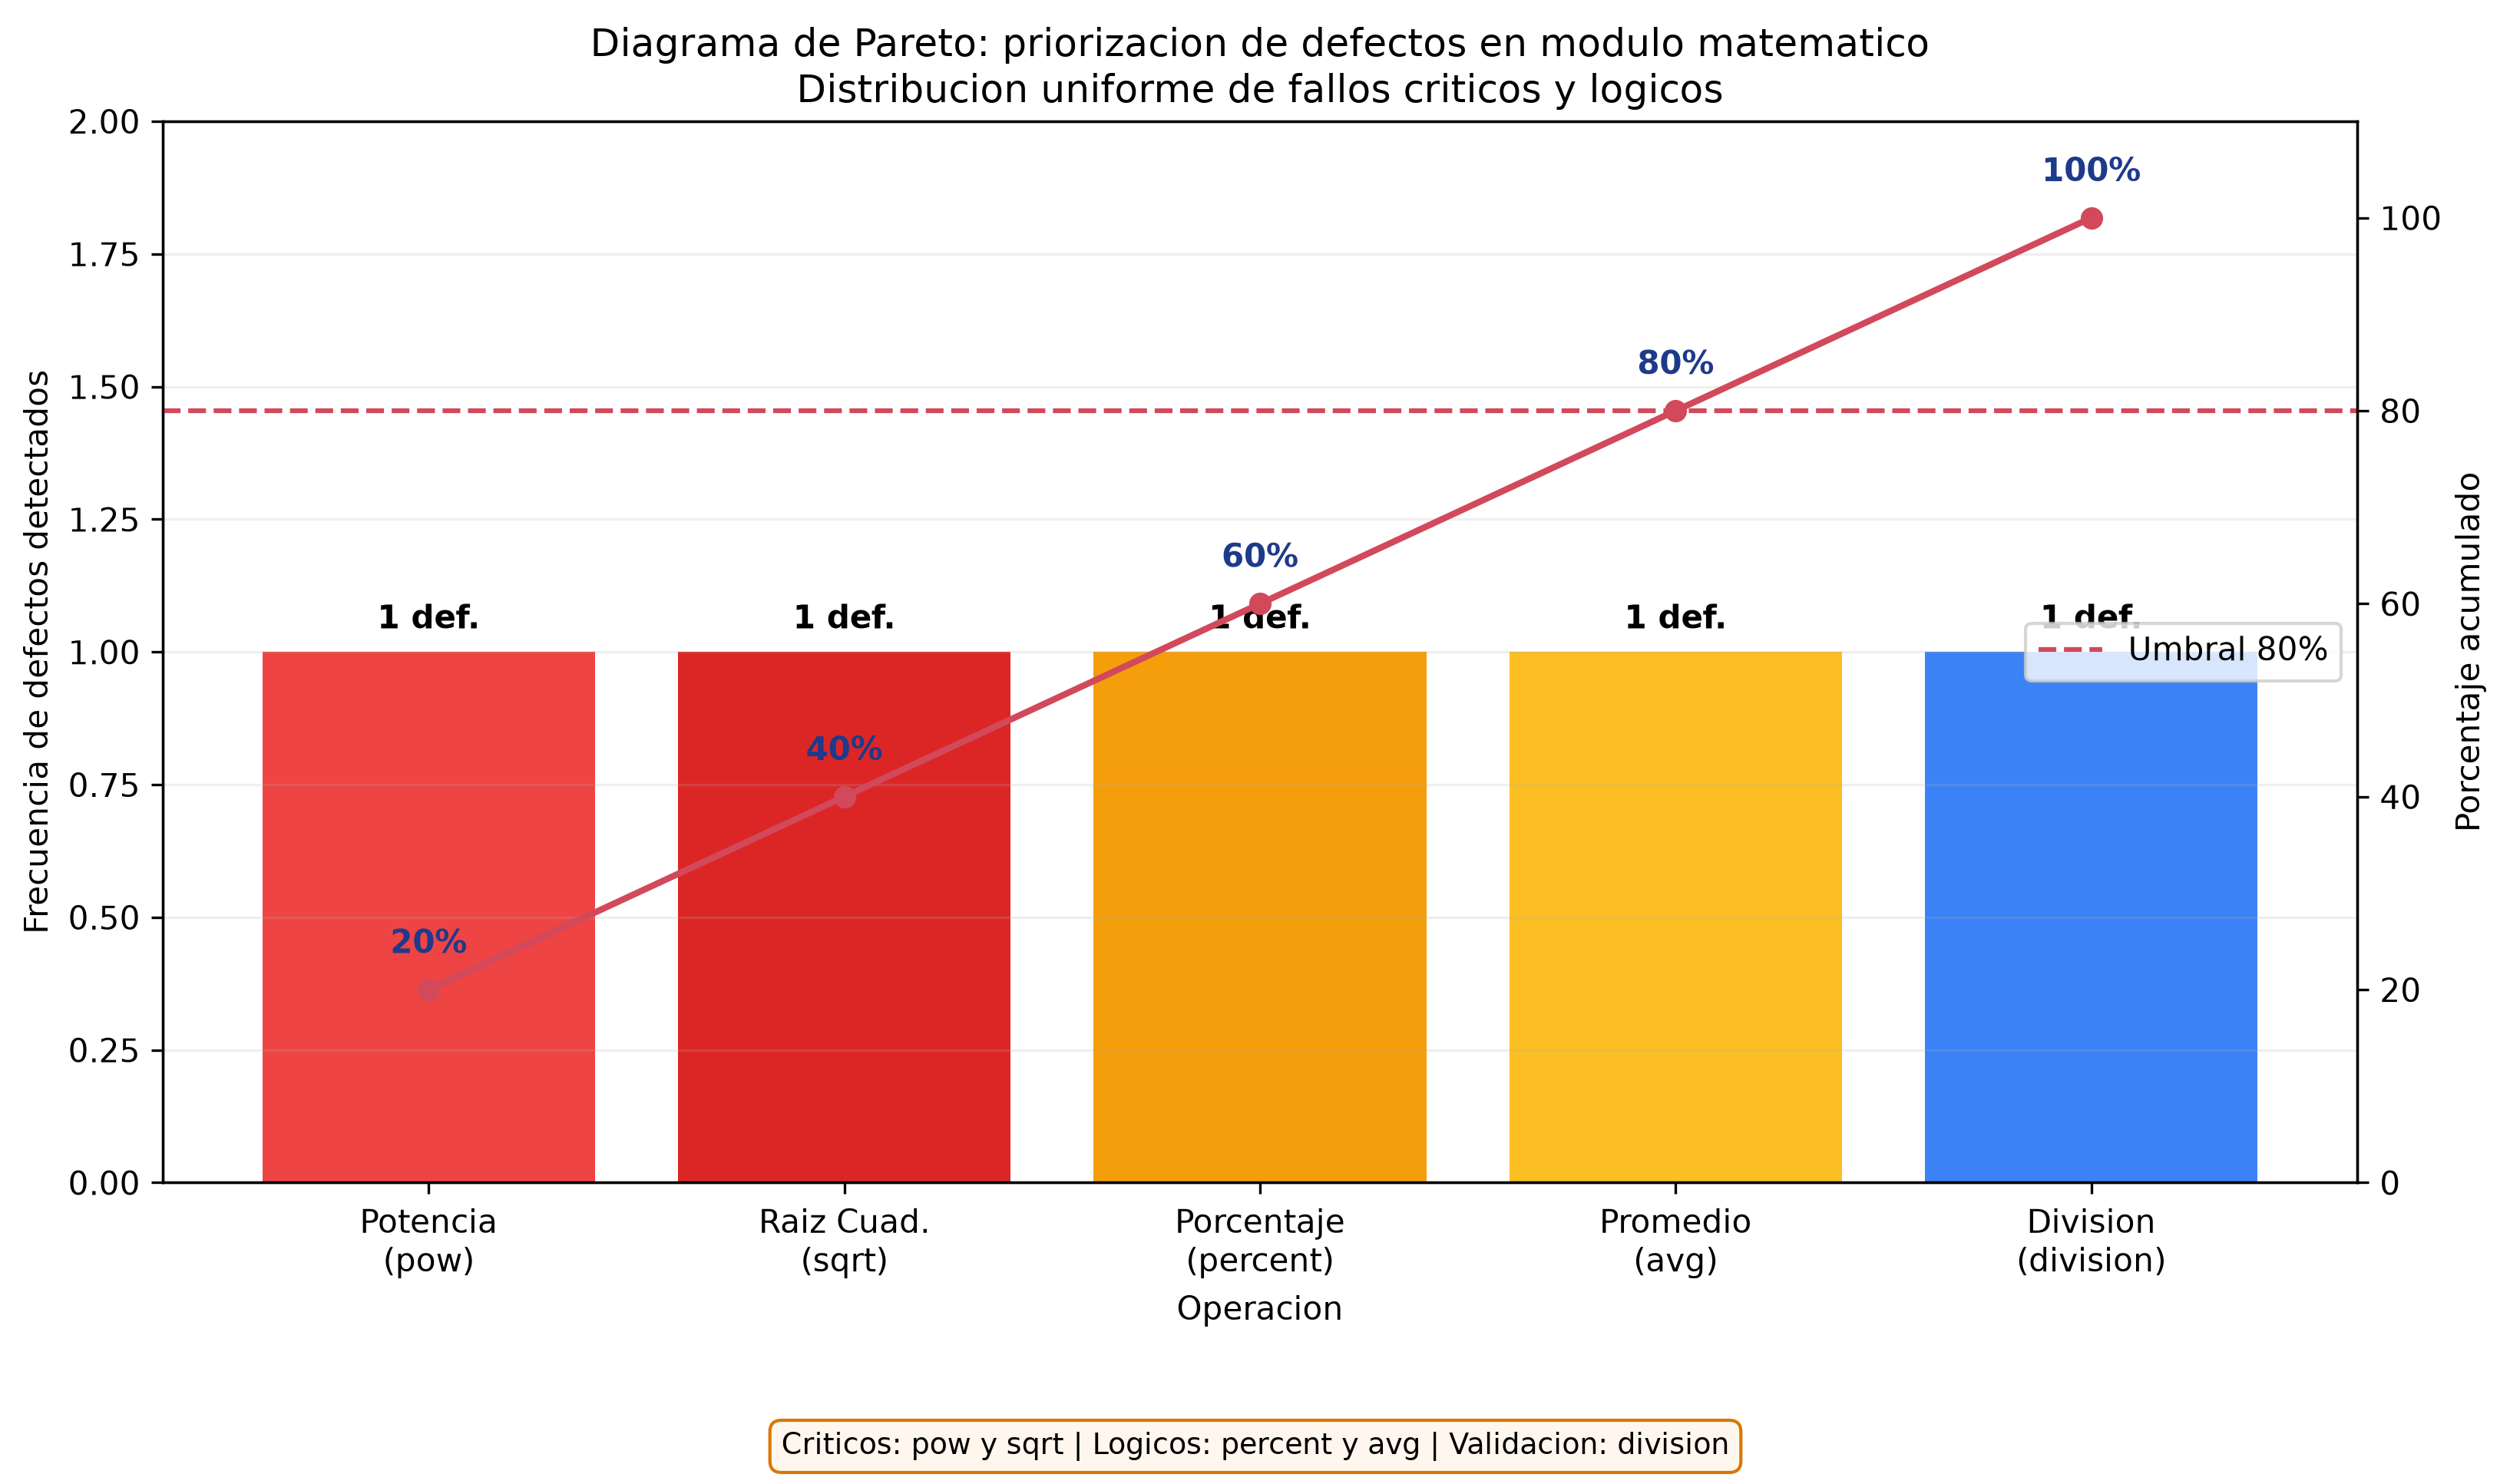
\includegraphics[width=0.98\textwidth]{resultados_calidad/pareto_operaciones.png}
\caption{Pareto de defectos con frecuencia, porcentaje acumulado y umbral del 80\%.}
\end{figure}

La interpretación correcta es que no existe una operación dominante. Las cinco operaciones deben ser atendidas porque presentan la misma frecuencia en el registro. Los colores diferencian fallos críticos de código, errores lógicos y errores de validación.

\section{Diagrama de Ishikawa}
El efecto analizado es: \textbf{errores en los resultados del módulo de operaciones}. Las causas fueron organizadas en cinco grupos:
\begin{itemize}[leftmargin=*]
  \item \textbf{Método:} fórmulas incompletas y claves inconsistentes.
  \item \textbf{Sistema/código:} diferencias entre \texttt{pow} y \texttt{power}, y ramas sin cobertura.
  \item \textbf{Persona:} revisión manual insuficiente e interpretación distinta de los requisitos.
  \item \textbf{Herramientas:} falta inicial de pruebas automatizadas y de pruebas de API.
  \item \textbf{Datos:} divisor cero, raíz negativa y porcentaje fuera de escala.
\end{itemize}

\begin{figure}[H]
\centering
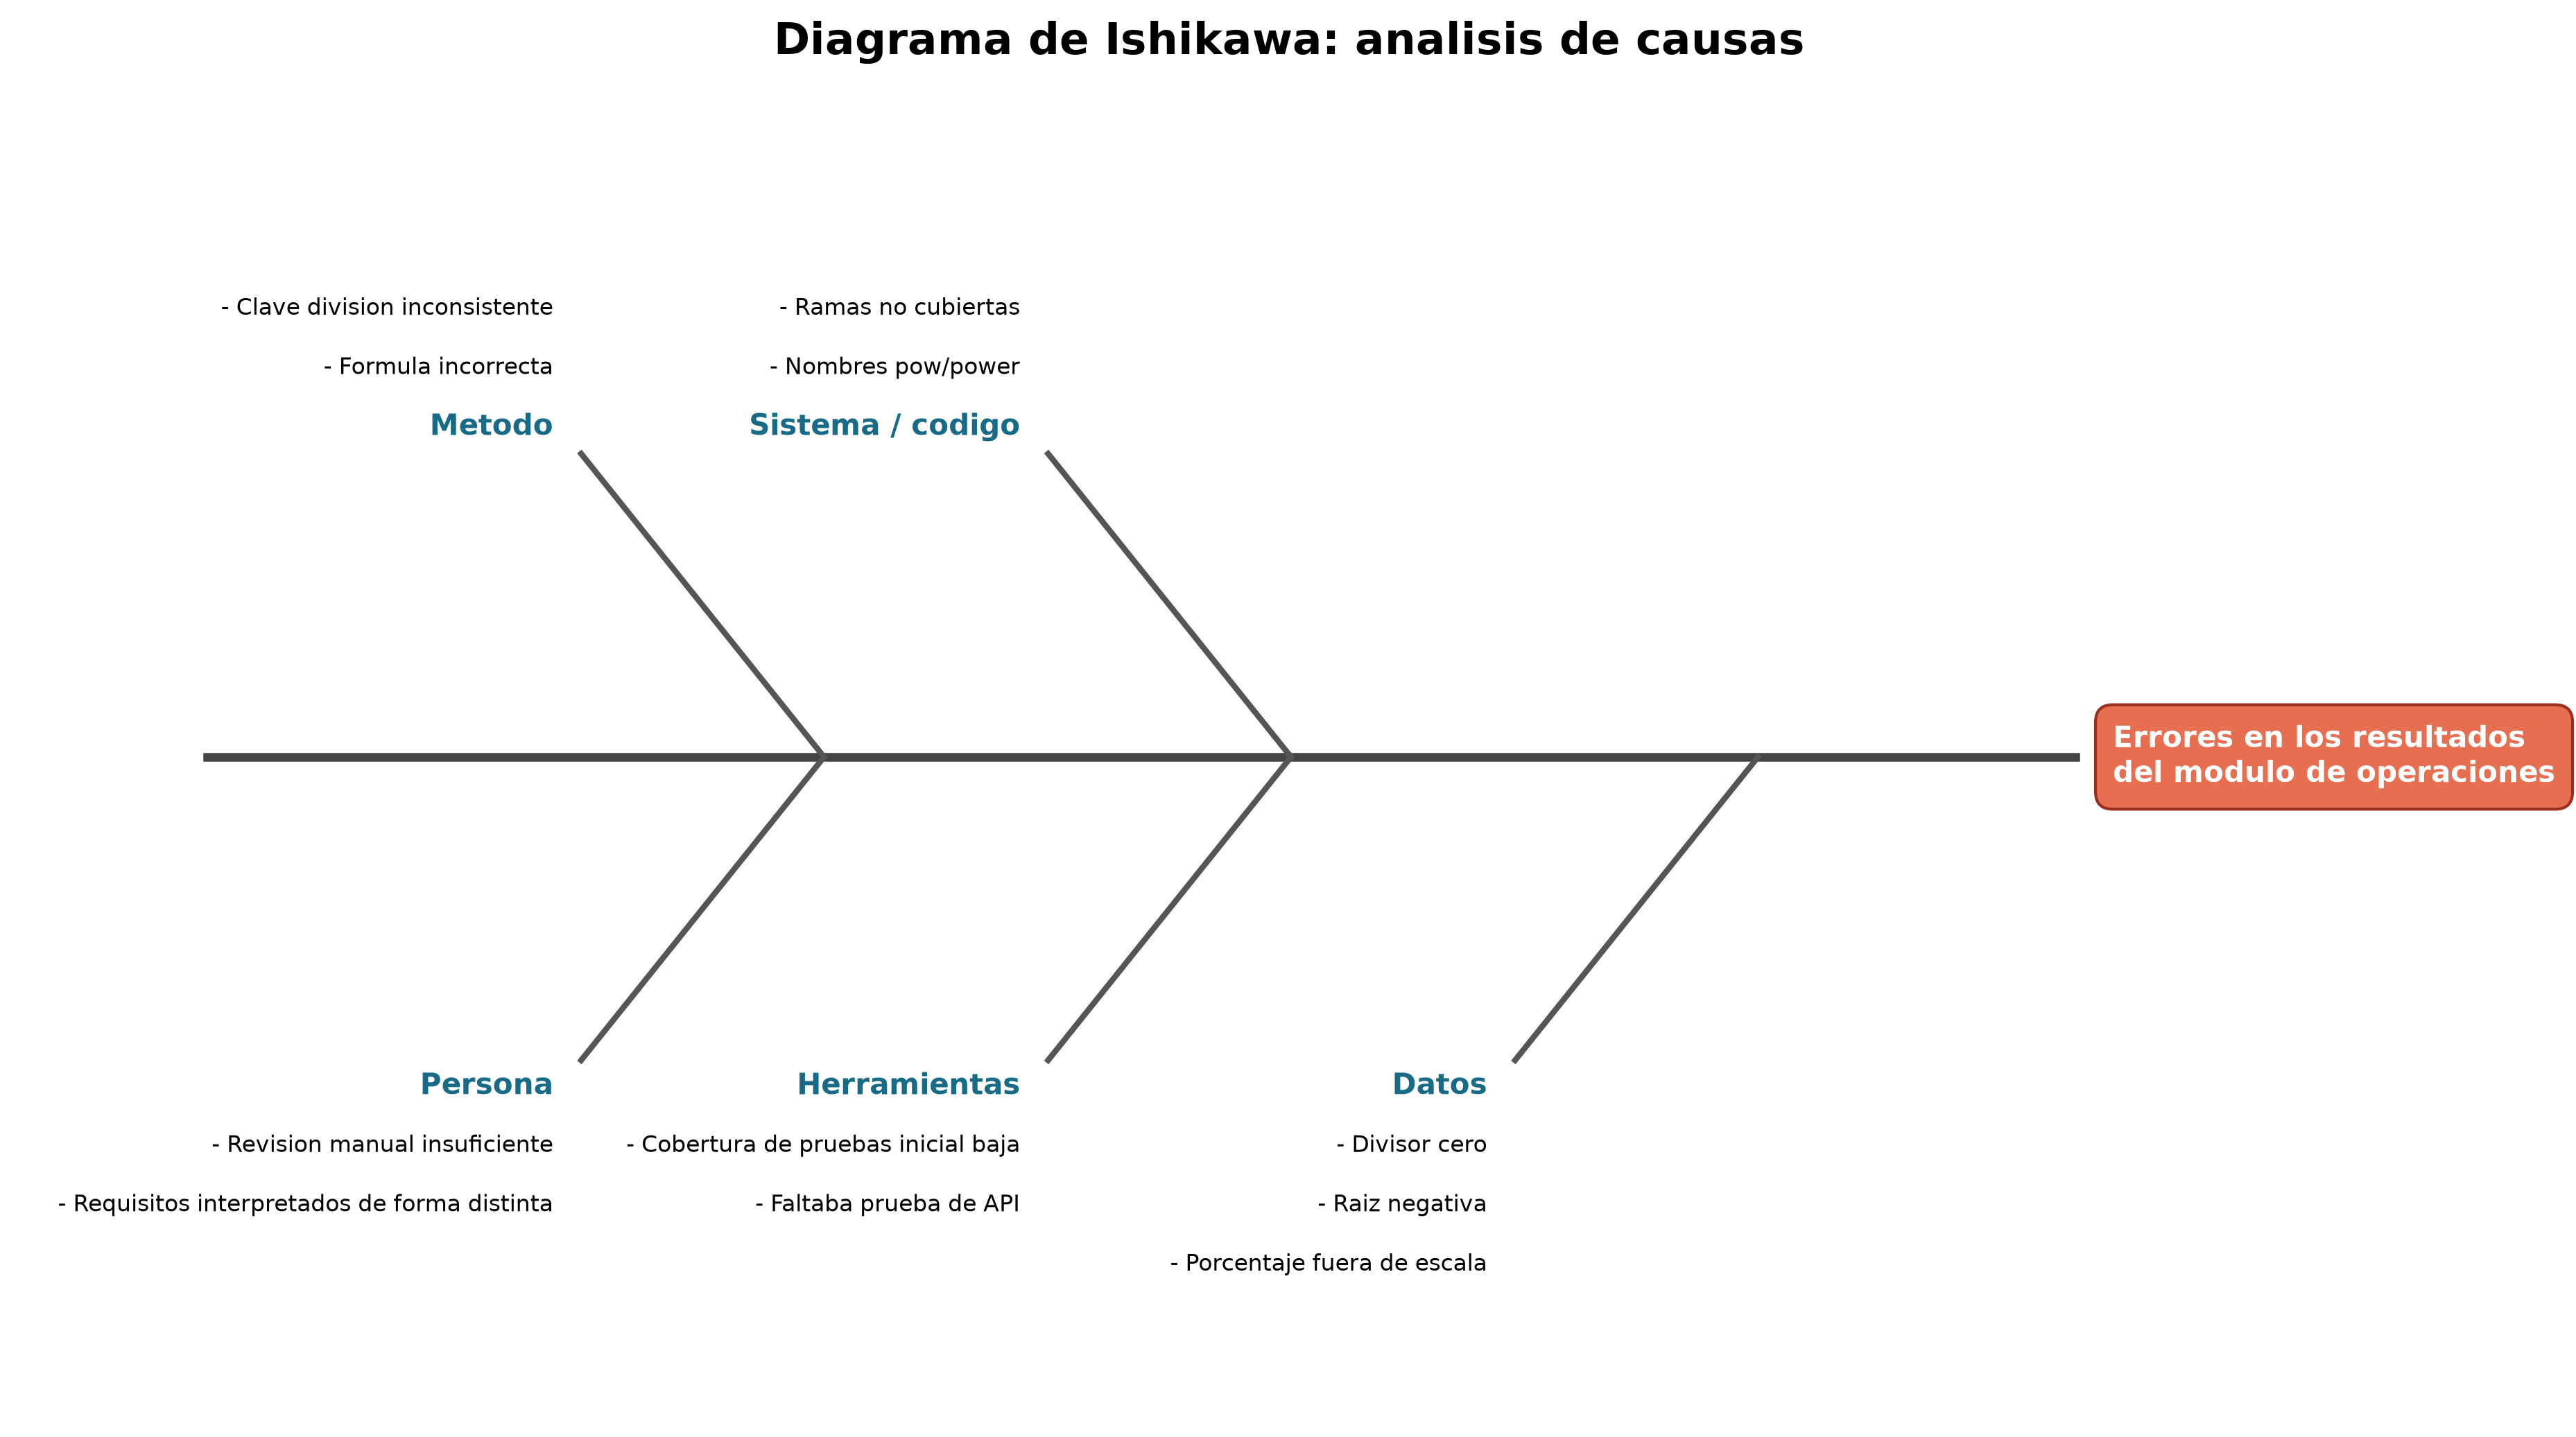
\includegraphics[width=0.98\textwidth]{resultados_calidad/ishikawa_operaciones.png}
\caption{Causas raíz de los errores del módulo.}
\end{figure}

Cada causa se relaciona con un hallazgo del registro. Por ejemplo, la fórmula incompleta se demuestra con el caso del porcentaje, mientras que el divisor cero y la raíz negativa se validan mediante pruebas de restricciones.

\section{Aplicación de PDCA}
La tabla PDCA completa se encuentra en \texttt{resultados\_calidad/tabla\_pdca.csv}.

\begin{longtable}{p{1.2cm}p{5cm}p{3cm}p{2.5cm}p{2.2cm}}
\caption{Aplicación del ciclo PDCA.}\\
\toprule
Etapa & Actividad & Indicador & Criterio & Resultado \\
\midrule
\endfirsthead
\toprule
Etapa & Actividad & Indicador & Criterio & Resultado \\
\midrule
\endhead
Plan & Definir errores en las cinco operaciones & Hallazgos & 5 casos delimitados & 5 casos \\
Do & Corregir nombres, fórmulas y validaciones & Correcciones & 5 correcciones & 5 aplicadas \\
Check & Ejecutar pruebas automatizadas & Fallos & 0 fallos & 0 de 11 \\
Act & Conservar pruebas y restricciones & Cobertura & 5 de 5 operaciones & 5 de 5 \\
\bottomrule
\end{longtable}

El ciclo no se presenta como una definición teórica: cada etapa tiene una actividad realizada, un indicador y un resultado comprobable.

\section{Aplicación de Six Sigma DMAIC}
La tabla completa se encuentra en \texttt{resultados\_calidad/tabla\_six\_sigma\_dmaic.csv}.

\begin{longtable}{p{1.4cm}p{5cm}p{3cm}p{2.5cm}p{2.2cm}}
\caption{Aplicación de Six Sigma DMAIC.}\\
\toprule
Etapa & Actividad & Indicador & Criterio & Resultado \\
\midrule
\endfirsthead
\toprule
Etapa & Actividad & Indicador & Criterio & Resultado \\
\midrule
\endhead
Define & Delimitar resultados incorrectos o no controlados & Alcance & 5 operaciones & 5 operaciones \\
Measure & Medir frecuencia, severidad e impacto & Hallazgos & 5 hallazgos & 5; 3 críticos; 2 altos \\
Analyze & Relacionar hallazgos con causas raíz & Causas & 100\% clasificados & 5 de 5 en Ishikawa \\
Improve & Corregir fórmulas, claves y validaciones & Correcciones & 5 correcciones & 5 aplicadas \\
Control & Repetir pruebas después de cada cambio & Pruebas fallidas & 0 fallos & 0 de 11 \\
\bottomrule
\end{longtable}

La medición confirma que el registro tiene cinco hallazgos, tres de severidad crítica y dos de severidad alta. El control se demuestra mediante la ejecución final de las once pruebas.

\section{Archivos y reproducibilidad}
Los archivos principales de la entrega son:
\begin{itemize}[leftmargin=*]
  \item \texttt{registro\_pruebas\_operaciones.csv}: evidencia de hallazgos y correcciones.
  \item \texttt{analisis\_taller\_operaciones.py}: generador de tablas y gráficos.
  \item \texttt{tabla\_errores\_encontrados.csv}: tabla detallada de defectos.
  \item \texttt{tabla\_pdca.csv}: tabla de mejora continua.
  \item \texttt{tabla\_six\_sigma\_dmaic.csv}: tabla DMAIC.
  \item \texttt{pareto\_operaciones.png}: priorización de hallazgos.
  \item \texttt{ishikawa\_operaciones.png}: análisis de causas.
\end{itemize}

Para regenerar las evidencias:
\begin{lstlisting}[language=bash]
/tmp/odoo16-analysis-venv/bin/python analisis_taller_operaciones.py
\end{lstlisting}

\section{Conclusiones}
\begin{enumerate}[leftmargin=*]
  \item Se identificaron cinco hallazgos asociados a las cinco operaciones analizadas.
  \item Se corrigieron inconsistencias de nombres, fórmulas, validaciones y cobertura de pruebas.
  \item El Pareto mostró una distribución uniforme: cada operación representa el 20\% de los hallazgos.
  \item El Ishikawa evidenció que las causas incluyen código, método, herramientas, persona y datos.
  \item PDCA y DMAIC se aplicaron con indicadores y resultados, no únicamente como conceptos teóricos.
  \item La verificación final produjo 11 pruebas ejecutadas, cero fallos y cero errores.
\end{enumerate}

\section{Guion breve para la defensa}
La explicación puede resumirse de la siguiente manera:

\begin{quote}
Se analizó el módulo de operaciones matemáticas de Odoo. Primero se registraron cinco hallazgos en división, promedio, potencia, raíz cuadrada y porcentaje. Después se corrigieron las claves inconsistentes, la fórmula de porcentaje, la validación de raíz negativa y la cobertura de pruebas. El Ishikawa permitió organizar las causas raíz y el Pareto mostró que los cinco tipos tienen la misma frecuencia. Finalmente se aplicaron PDCA y DMAIC con indicadores medibles. La solución se verificó ejecutando once pruebas de Odoo, con cero fallos y cero errores.
\end{quote}

\bibliographystyle{IEEEtran}
\bibliography{biblio}
\nocite{*}

\end{document}
